\chapter{Revisión de la Literatura}
  \section{Redes Neuronales Artificiales}
  
    Las redes neuronales artificiales (RNA) son modelos computacionales de la Inteligencia Artificial los cuales contienen simples unidades de procesamientos llamadas neuronas.  Ellas se inspiran en el cerebro humano, tomando como base la conectividad entre neuronas y el aprendizaje que pueden tener.  Un perceptron o neurona (artificial) solamente resuelve problemas lineales y tiene la siguiente forma:
    
    \begin{figure}[H]
      \centering
      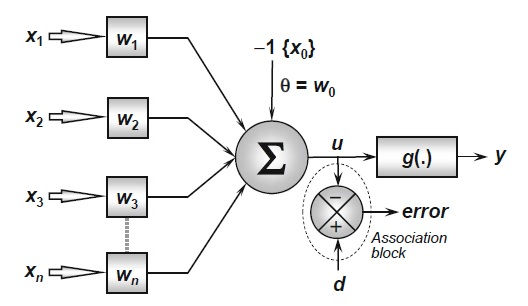
\includegraphics[width=\columnwidth]{ANN.jpg}
      \caption{Red Neuronal Artificial B\'asica}
      \label{fig:fig1}
    \end{figure}

    Donde $\Sigma$ es la representación matemática de la neurona.,  $x_1$, $x_2$,  \dots  ,$x_n$ son las variables de entrada a la red.  $w_1$,$w_2$,  \dots , $w_n$ son los pesos con los cuales se van a podnerar las entradas, es decir multiplicar cuando la información entra en la neurona. Posterior a multiplicar el peso por la entrada correspondiente,  se suman todos esos valores $w_1$$x_1$ + $w_2$$x_2$ + $w_3$$x_3$.

